\chapter{Introduction au domaine}

\section{Modèles}
Le principal modèle développé est celui des créatures.
Ce modèle permet de simuler l'évolution d'une espèce dans un milieu donné.
Il utilisera le réseau de neurones comme ``attribut de classe''.\\
Les individus (les créatures) doivent pour survivre, boire de l'eau, éviter le feu et ramener des diamants à la maison.
\\Pour bouger, la créature a la possibilité de détecter si :\\

\begin{itemize}
 \item un diamant est devant elle
 \item de l'eau est devant elle
 \item du feu est devant elle
 \item la maison est devant elle
 \item elle transporte actuellement un diamant\\
\end{itemize}

En sortie, la créature à le choix de :
\begin{itemize}
 \item tourner à gauche
 \item tourner à droite
 \item avancer
 \item ne rien faire\\
 
\end{itemize}
 
Le choix des actions est déterminé par les poids attribués à chaque signal au sein du réseau de neurones associé à la créature.\\

Dans un second temps, un modèle basé sur la bourse (ex: CAC40) est envisagé.
Il utilisera aussi le réseau de neurones déjà implémenté.
\clearpage




\section{Réseau de neurones}

Dans le domaine de la science cognitive et de l'apprentissage automatique, les réseaux de neurones artificiels sont une famille d'algorithmes d'apprentissage statistique inspirés par les réseaux de neurones biologiques (système nerveux central, cerveau) et sont utilisés pour estimer ou approximer une fonction pouvant prendre un nombre important d'entrées généralement inconnues.\\

L'élément clé de ce paradigme réside dans la structure particulière du système de traitement de l'information. Il est habituellement composé d'un large nombre d'éléments de traitement interconnectés, neurones, travaillant à l’unisson afin de résoudre un problème spécifique. Un réseau de neurones apprend par l'exemple et est configuré pour une application spécifique telle que la reconnaissance de forme ou la classification de données au travers d'un processus dit d’apprentissage. Ce processus, dans un système nerveux biologique, implique l'ajustement des connexions synaptiques existantes entre les neurones, ce qui est vrai également dans un réseau artificiel.

   


\subsection{Le Neurone Artificiel}

\begin{figure}[H]
    \centering
    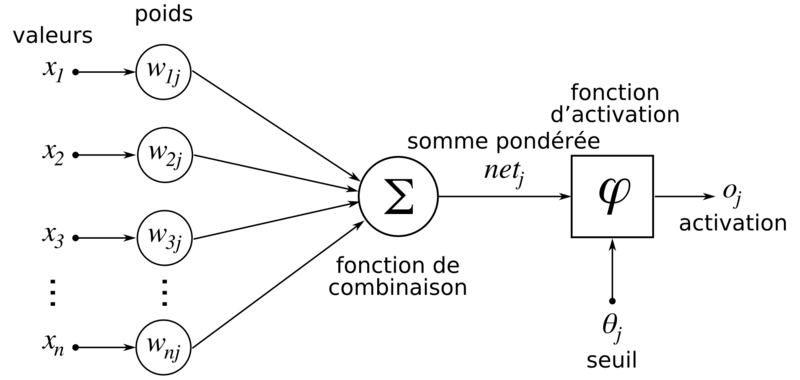
\includegraphics[width=\textwidth]{./pictures/800px-ArtificialNeuronModel_francais.png}
    \caption{Structure d'un neurone artificiel. Le neurone calcule la somme de ses entrées puis cette valeur passe à travers la fonction d'activation pour produire sa sortie.}
\end{figure}
Un neurone artificiel est une unité de traitement qui reçoit des données en entrée, sous la forme d’un vecteur, et produit une sortie réelle. Cette sortie est déterminée en fonction des valeurs d'entrées et des poids des connexions.\\


La valeur numérique du poids associé à une connexion entre deux unités reflète la force de la relation entre ces deux unités. Si cette valeur est positive, la connexion est dite excitatrice, sinon elle est dite inhibitrice.


\subsection{Réseau de neurones}

Un réseau de neurones est en général composé d'une succession de couches dont chacune prend ses entrées sur les sorties de la précédente. Chaque couche $(i)$ est composée de $N_{i}$ neurones, prenant leurs entrées sur les $N_{i-1}$ neurones de la couche précédente. À chaque synapse est associée un poids synaptique, de sorte que les $N_{i-1}$ sont multipliés par ce poids, puis additionnés par les neurones de niveau $i$, ce qui est équivalent à multiplier le vecteur d'entrée par une matrice de transformation. Mettre l'une derrière l'autre les différentes couches d'un réseau de neurones reviendrait à mettre en cascade plusieurs matrices de transformation et pourrait se ramener à une seule matrice, produit des autres, s'il n'y avait à chaque couche, la fonction de sortie qui introduit une non linéarité à chaque étape.\\
Ceci montre l'importance du choix judicieux d'une bonne fonction de sortie : un réseau de neurones dont les sorties seraient linéaires n'aurait aucun intérêt.

\begin{figure}[H]
    \centering
    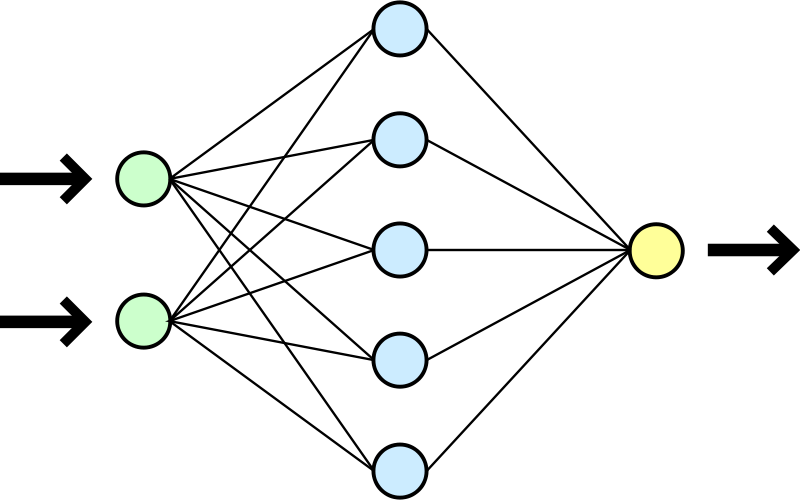
\includegraphics[width=0.8\textwidth]{./pictures/800px-Neural_network.png}
    \caption{Vue simplifiée d'un réseau artificiel de neurones.}
\end{figure}

\subsection{Fonction de combinaison}

Considérons un neurone quelconque.

Il reçoit des neurones en amont un certain nombre de valeurs via ses connexions synaptiques, et il produit une certaine valeur en utilisant une \textbf{fonction de combinaison}. Cette fonction peut donc être formalisée comme étant une fonction vecteur-à-scalaire, notamment :

\begin{itemize}
    \item[$\bullet$] Les réseaux de type \textbf{MLP} (Multi-Layer Perceptron) calculent une combinaison linéaire des entrées, c’est-à-dire que la fonction de combinaison renvoie le produit scalaire entre le vecteur des entrées et le vecteur des poids synaptiques.
    \item[$\bullet$] Les réseaux de type \textbf{RBF} (Radial Basis Function) calculent la distance entre les entrées, c’est-à-dire que la fonction de combinaison renvoie la norme euclidienne du vecteur issu de la différence vectorielle entre les vecteurs d’entrées.
\end{itemize}

\subsection{Fonction d’activation}
La \textbf{fonction d’activation} (ou fonction de seuillage) sert à introduire une non-linéarité dans le fonctionnement du neurone.


Les fonctions de seuillage présentent généralement trois intervalles :
\begin{enumerate}
    \item en dessous du seuil, le neurone est non-actif (souvent dans ce cas, sa sortie vaut 0 ou -1) ;
    \item aux alentours du seuil, une phase de transition ;
    \item au-dessus du seuil, le neurone est actif (souvent dans ce cas, sa sortie vaut 1).
\end{enumerate}



\section{Algorithme génétique}
Les algorithmes génétiques s'inspirent de l'évolution des espèces. Leur but est de trouver une solution tendant vers l'optimal, en un temps raisonnable. Ils vont à partir d'un problème donné, chercher une solution selon le processus suivant: 

\begin{itemize}
    \item création d'une population initiale ayant des caractéristiques aléatoires
    \item évaluation de la population
    \item sélection, reproduction, mutation
    \item insertion des nouveaux individus dans la population
    \item évaluation de la nouvelle génération, sélection, reproduction, etc...\\
\end{itemize}


\subsection{Création de la population initiale}

	Au début de notre programme, la population est créée aléatoirement: c'est-à-dire que les gènes attribués aux individus sont aléatoires. Cette population ne répondra pas forcément aux critères de sélection, elle devra cependant être cohérente par rapport à son environnement. Par exemple, si l'on code un jeu, ces individus devront respecter les règles du jeu, mais ne donneront pas forcément une solution au problème.\\

\subsection{Evaluation de la population}

	Notre population initiale étant créée, cette étape consiste maintenant à évaluer les individus dans leur environnement selon plusieurs critères définis et à leur attribuer un score.\\

\subsection{Sélection, reproduction, mutation}

	Cette étape permet la création d'une nouvelle génération: nous allons tout d'abord sélectionner les différents individus qui seront ensuite utilisés pour la création d'une nouvelle génération, nous allons ensuite croiser leurs gènes. Enfin une mutation peut être introduite chez certains individus de la nouvelle génération.
 
	Il existe plusieurs modes de sélection d'individus :
	\begin{itemize}
	\item Sélection par roulette : probabilité de sélection proportionnelle à leurs performances, il y a cependant un risque de surreprésentation.
	\item Sélection par rang : chromosomes triés par leurs performances, la probabilité de sélection dépend du rang du chromosome, et non plus des performances, ce qui évite d'avoir une surreprésentation.
	\item Sélection par tournoi : on crée m paires de chromosomes à partir de m chromosomes, on fixe alors une probabilité de sélection plus importante (entre 70\% et 80\%) pour le plus fort. 
	\item Sélection steady-state : une grande partie de la population est conservée, les plus mauvais sont remplacés par des nouveaux, produits à partir des meilleurs individus.
	\item Elitisme : reproduction à l'identique des meilleurs chromosomes afin d'éviter de les perdre lors de la reproduction.\\
	\end{itemize}
	
	
	Le croisement des gènes des individus peut se faire aléatoirement, cependant il existe une solution qui est largement plus répendue: les croisements multi-points. Le croisement multi-point consiste à découper en N morceaux les gènes de chaque individu choisi, puis à coupler ces gènes entre eux pour en créer un nouveau.\\
	\begin{figure}[H]

	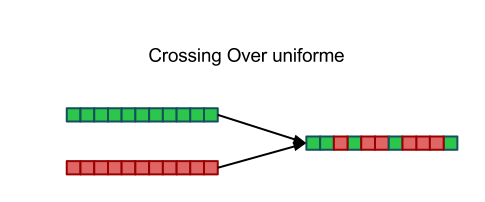
\includegraphics[width=0.5\textwidth]{./pictures/reproduction.png}
	
	\caption{Croisement de deux gènes}
	\end{figure}
	Enfin, la mutation génétique consiste à appliquer à certains individus (un très faible pourcentage), de façon aléatoire,une substitution d'un gène par un autre.\\
	\begin{figure}[H]

	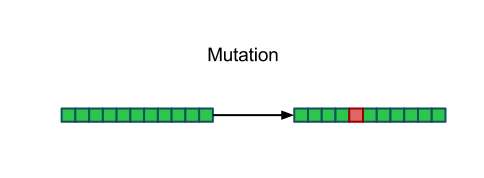
\includegraphics[width=0.5\textwidth]{./pictures/mutation.png}
	
	\caption{Mutation}
	\end{figure}
	

	Une fois la nouvelle génération créée et son cycle de vie terminé, on lui applique les mêmes tests d'évaluation et modes de sélection que la génération précédente.

Le programmeur peut choisir le nombre de génération à créer: généralement, une solution est trouvée en moins de 10 générations, et au bout de 500 générations, les solutions n'évoluent plus, cependant rien ne garantit que nous obtenions une solution optimale.

Nous pouvons donc en conclure que les algorithmes génétiques offrent une grande liberté de paramétrage et d'implémentation au programmeur, ce qui en fait un outil utilisé dans plusieurs domaines de recherche.

